% http://users.ece.northwestern.edu/~sda690/MfB/Motion_CVPR08.pdf
% https://www.geeksforgeeks.org/opencv-motion-blur-in-python/
% https://www.wikiwand.com/en/Motion_blur
% http://tech.abdulfatir.com/2014/05/kernel-image-processing.html

Além dos filtros de \textit{blur} apresentados na \hyperref[sec:blur]{seção anterior}, temos também um filtro de \textit{blur} direcionado, muitas vezes usado para alcançar um efeito de \textit{motion blur}. Para o \textit{kernel} da \cref{fig:h9}, o \textit{blur} está direcionado a 45\textdegree, como se a câmera estivesse se movendo da esquerda-superior para a direita-inferior, ou vice-versa.

\begin{figure}[H]
    \centering
    \begin{kmatrix}
    \matrix(img)[square matrix]{
        1 & 0 & 0 & 0 & 0 & 0 & 0 & 0 & 0 \\
        0 & 1 & 0 & 0 & 0 & 0 & 0 & 0 & 0 \\
        0 & 0 & 1 & 0 & 0 & 0 & 0 & 0 & 0 \\
        0 & 0 & 0 & 1 & 0 & 0 & 0 & 0 & 0 \\
        0 & 0 & 0 & 0 & 1 & 0 & 0 & 0 & 0 \\
        0 & 0 & 0 & 0 & 0 & 1 & 0 & 0 & 0 \\
        0 & 0 & 0 & 0 & 0 & 0 & 1 & 0 & 0 \\
        0 & 0 & 0 & 0 & 0 & 0 & 0 & 1 & 0 \\
        0 & 0 & 0 & 0 & 0 & 0 & 0 & 0 & 1 \\
    };

    \node[left=of img] {$\displaystyle\Scale[1.7]{\frac{1}{9}}$};
\end{kmatrix}

    \caption{Máscara de \textit{motion blur}: $h_9$.}
    \label{fig:h9}
\end{figure}

\begin{figure}[H]
    \centering
    \begin{subfigure}{0.48\textwidth}
        \centering
        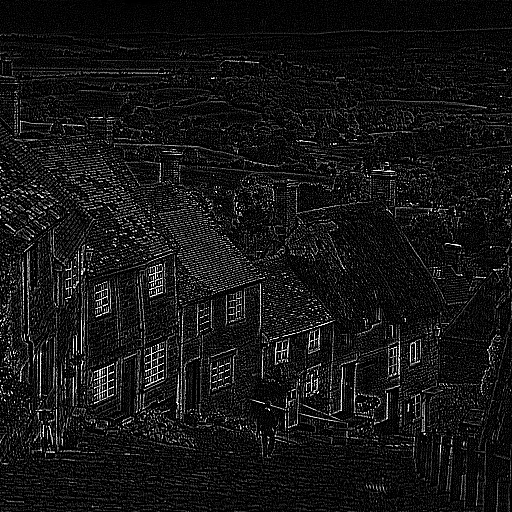
\includegraphics[width=0.9\textwidth]{imagens/city.png}
        \caption{Original: \texttt{city.png}.}
    \end{subfigure}%
    \begin{subfigure}{0.48\textwidth}
        \centering
        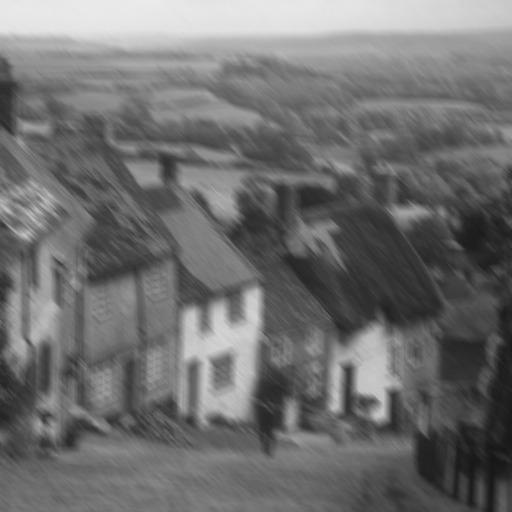
\includegraphics[width=0.9\textwidth]{resultados/city_h9.png}
        \caption{Convolução com $h_9$ (\ref{fig:h9}).}
        \label{fig:motion:conv}
    \end{subfigure}

    \caption{Aplicação de \textit{motion blur}.}
    \label{fig:motion}
\end{figure}

Para a execução pelo programa, o comando deve ser no formato abaixo, resultando em algo como a \cref{fig:motion:conv}.

\begin{minted}{bash}
    $ python3 main.py imagens/city.png h9
\end{minted}

